\chapter{Asking Millionaire Homeowners How They Got Rich}

These companion notes follow a School of Hard Knocks interview, curated by LazyingArt LLC, and the lecture must be read in the order in which it is staged. We begin with houses, a Ferrari, and giant money claims before we are given any clean distinction between exit value, annual revenue, projected revenue, or personal wealth. Only afterward does the lecture earn its way toward mechanism: access, retail economics, bootstrapping, allocation, delegation, selling, creative financing, and finally the harder question of what money cannot repair. No validated mathematical screenshots survive for this lecture, so every displayed relation and every figure below is transcript-led rather than frame-led.

\section{Cold Open: Giant Numbers and Wrong Units}

The lecture opens with theater. A homeowner says that he sold a company for \$235 million; another speaker moves from an ``almost \$100 billion'' sale claim to \$850 million for the year and then to a projected billion-dollar year. The opening is supposed to dazzle us, but it also obliges us to separate economic objects before we confuse them.

\begin{table}[h]
\centering
\caption{The opening ledger: unlike quantities must not be merged}
\begin{tabular}{|l|l|l|}
\hline
Speaker claim & Quantity type & Source-conscious reading \\
\hline
``I sold my last company for \$235 million'' & exit value & relatively stable transcript claim \\
``We did \$850 million for the year'' & annual company revenue / sales & operating flow, not sale price \\
``We're going to do a billion this year'' & targeted annual revenue / sales & projected flow, not realized wealth \\
``\$235 billion'', ``almost \$100 billion'' & unstable large-number talk & likely joking, garbled, or inflated \\
\hline
\end{tabular}
\end{table}

We therefore begin with a strict notation:
\begin{align}
S_{\mathrm{exit},1} &= 235\times 10^{6}\ \mathrm{USD},\\
R_{\mathrm{yr},1} &= 850\times 10^{6}\ \mathrm{USD},\\
R_{\mathrm{target},1} &= 10^{9}\ \mathrm{USD}.
\end{align}

This is the first important discipline of the chapter. The lecture wants us to feel aspiration and confusion at the same time; the notes must preserve the feeling but remove the bookkeeping error. The governing question is then stated in blunt form: how does somebody become a multimillionaire in today's world? At this point the lecture does not answer. It only points us toward the field in which an answer might be found.

\section{Boca Raton as an Access Problem}

The next move is not about business at all. It is geographical and social. ``Everyone thinks Miami is where the money is,'' the host says, but if we want quiet wealth rather than visible performance, we go north to Boca Raton. That pivot matters because the lecture's first real mechanism is not finance; it is access.

The host door-knocks, rings bells, speaks through intercoms, gets turned away, gets interrupted, and keeps going. The refusals are not dead air. They are the lecture's first model of method. If one approach has some success probability \(p_{\mathrm{yes}}\), and if \(Y_n\) denotes the number of usable interviews obtained after \(n\) attempts, then the host's motto, ``volume negates luck,'' can be compressed into
\begin{align}
E[Y_{n+1}] &= E[Y_n] + p_{\mathrm{yes}},\\
E[Y_n] &= n\,p_{\mathrm{yes}}.
\end{align}
This is a cautious reconstruction, not a measured social law. But it captures the lecture's exact rhythm: every no is a step closer to a yes because each refusal is one more trial completed.

\begin{figure}[h]
\centering
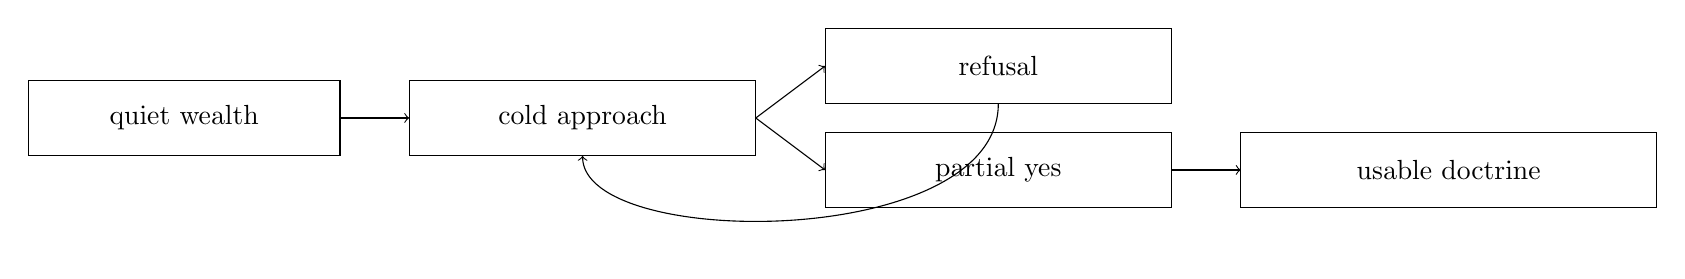
\begin{tikzpicture}[x=2.2cm,y=1.2cm]
\draw (0,0) rectangle (1.8,0.8);
\node at (0.9,0.4) {quiet wealth};

\draw (2.2,0) rectangle (4.2,0.8);
\node at (3.2,0.4) {cold approach};

\draw (4.6,0.55) rectangle (6.6,1.35);
\node at (5.6,0.95) {refusal};

\draw (4.6,-0.55) rectangle (6.6,0.25);
\node at (5.6,-0.15) {partial yes};

\draw (7.0,-0.55) rectangle (9.4,0.25);
\node at (8.2,-0.15) {usable doctrine};

\draw[->] (1.8,0.4) -- (2.2,0.4);
\draw[->] (4.2,0.4) -- (4.6,0.95);
\draw[->] (4.2,0.4) -- (4.6,-0.15);
\draw[->] (6.6,-0.15) -- (7.0,-0.15);
\draw[->] (5.6,0.55) .. controls (5.6,-1.0) and (3.2,-1.0) .. (3.2,0);
\end{tikzpicture}
\caption{A transcript-led funnel for access: not every attempt yields a theory, but repeated attempts occasionally produce one}
\end{figure}

The lecture is careful not to romanticize persistence too quickly. Some interactions end with a clean refusal. Others yield only fragments: a husband in private equity, a short line about working hard, a note on values, and the insistence that the right life partner is chosen through shared moral structure. These are not full business doctrines, but they are not useless. They tell us that the field is real even when entry remains partial.

\subsection{Question \& Answer}

\paragraph{Question.} How does access actually work in a field where almost everyone says no?

\paragraph{Answer.} By changing the unit of analysis. A refusal is not yet information about our final chances; it is merely one completed trial. The host's pedagogy is therefore probabilistic before it becomes entrepreneurial. First we survive the refusal structure. Only then do we get to learn from wealth.

\section{From \$10{,}000 to \$100 Million: Store-by-Store Scale}

After the refusals, the lecture earns its first long mechanism. A founder says he built the world's largest e-cigarette brand in under five years with \$10{,}000, reached a \$100 million year, hit \(100{,}000\) points of distribution, broke \$100 million in \(18\) months, and later sold the company. The order matters. The lecture does not start with branding. It starts with the street, the store, and the counter.

The quantitative skeleton is compact:
\begin{align}
K_{\mathrm{boot,e\mbox{-}cig}} &= 10{,}000\ \mathrm{USD},\\
R_{\mathrm{yr},\mathrm{e\mbox{-}cig}}^{\mathrm{peak}} &= 100\times 10^{6}\ \mathrm{USD},\\
D_{\mathrm{e\mbox{-}cig}} &= 100{,}000,\\
R_{18\mathrm{m},\mathrm{e\mbox{-}cig}} &\ge 100\times 10^{6}\ \mathrm{USD}.
\end{align}

The founder's selling language is highly charged. He pitches the product on smell, social convenience, and health rhetoric. We keep that language only as speaker-reported sales talk. The lecture's real mechanism is not the rhetoric itself but the economic structure underneath it: trial, margin, guarantee, reorder.

The cleanest arithmetic in the lecture appears when the founder explains the disposable product. It sells for \$9.99; the store pays \$5.95; the store makes ``40\% gross profit.'' Let
\[
P_{\mathrm{retail}}=9.99\ \mathrm{USD},\qquad C_{\mathrm{store}}=5.95\ \mathrm{USD}.
\]

\paragraph{Worked Example.} The gross-profit calculation proceeds exactly in the order spoken by the interview.
\begin{enumerate}
\item Subtract the store's cost from the retail price:
\[
G_{\mathrm{store}}=P_{\mathrm{retail}}-C_{\mathrm{store}}=9.99-5.95=4.04\ \mathrm{USD}.
\]
\item Convert dollar profit to margin:
\[
m_{\mathrm{store}}=\frac{G_{\mathrm{store}}}{P_{\mathrm{retail}}}
=\frac{9.99-5.95}{9.99}.
\]
\item Evaluate numerically:
\[
m_{\mathrm{store}}\approx 0.4044.
\]
\item Compare with the transcript:
\[
0.4044 \approx 40.44\%,
\]
which is very close to the speaker's quoted ``40\% GP.''
\end{enumerate}

The lecture then takes a second step. The founder says that rechargeables were defective, expensive, and burdened by returns. So the business problem is not merely to sell an e-cigarette. It is to reduce failure, reduce cost, improve retailer economics, and make the consumer's choice easy enough to happen quickly at the counter.

\begin{figure}[h]
\centering
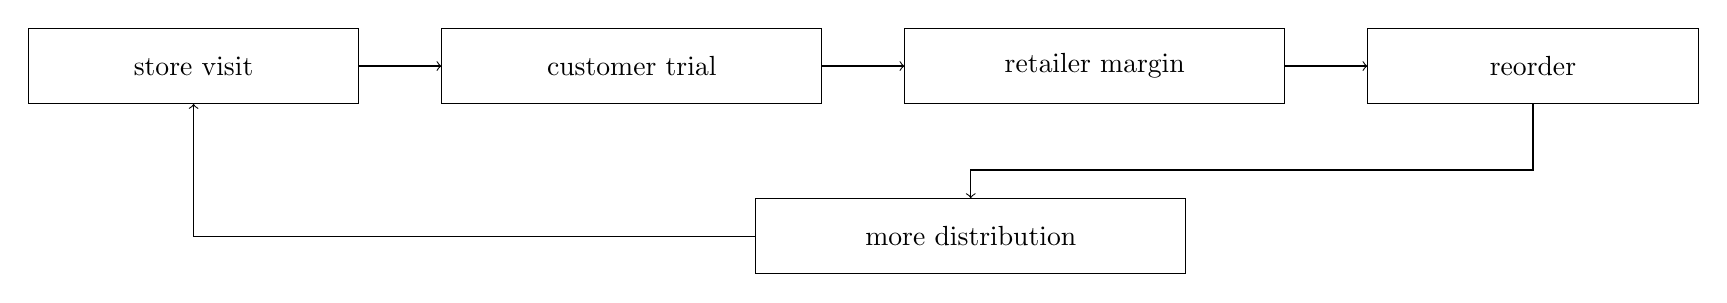
\begin{tikzpicture}[x=2.1cm,y=1.2cm]
\draw (0,0) rectangle (2.0,0.8);
\node at (1.0,0.4) {store visit};

\draw (2.5,0) rectangle (4.8,0.8);
\node at (3.65,0.4) {customer trial};

\draw (5.3,0) rectangle (7.6,0.8);
\node at (6.45,0.4) {retailer margin};

\draw (8.1,0) rectangle (10.1,0.8);
\node at (9.1,0.4) {reorder};

\draw (4.4,-1.8) rectangle (7.0,-1);
\node at (5.7,-1.4) {more distribution};

\draw[->] (2.0,0.4) -- (2.5,0.4);
\draw[->] (4.8,0.4) -- (5.3,0.4);
\draw[->] (7.6,0.4) -- (8.1,0.4);
\draw[->] (9.1,0) -- (9.1,-0.7) -- (5.7,-0.7) -- (5.7,-1.0);
\draw[->] (4.4,-1.4) -- (1.0,-1.4) -- (1.0,0.0);
\end{tikzpicture}
\caption{A transcript-led scale loop: guarantee and margin induce retailer acceptance; trial induces reorder; reorder expands distribution}
\end{figure}

The simplification move is one of the best practical moments in the lecture. The founder places plain white boxes on the counter and writes familiar cigarette identities on the outside, thereby mapping an overfull category back to an existing smoker identity. The four nicotine markers are given only as spoken values,
\[
N=\{2.7,\,1.8,\,1.5,\,<1\},
\]
and we deliberately do not assign units the transcript does not supply.

\begin{table}[h]
\centering
\caption{The white-box simplification map}
\begin{tabular}{|l|l|}
\hline
Outer label written on box & Guided product choice inside the Logic line \\
\hline
Marlboro & Logic Platinum \\
Marlboro Light & Logic Gold Label \\
Newport & corresponding Logic choice indicated, exact line not stably specified \\
\hline
\end{tabular}
\end{table}

The lecture now adds a branding maneuver. The founder distinguishes, in his own speaker-reported way, between making a literal claim and naming a brand. He cites the ``five hour energy'' example and says he borrowed that logic to position Logic as ``the most trusted brand.'' We should not mistake this for legal doctrine. It is the interviewee's business rhetoric about trademark leverage.

\begin{figure}[h]
\centering

\begin{tikzpicture}[x=2.6cm,y=1.2cm]
\draw (0,0) rectangle (2.8,1.0);
\node at (1.4,0.65) {literal claim};
\node at (1.4,0.35) {``fact about product''};

\draw (4.0,0) rectangle (7.3,1.0);
\node at (5.65,0.65) {brand positioning};
\node at (5.65,0.35) {trademarked phrase};

\draw[->] (2.8,0.5) -- (4.0,0.5);
\node at (3.4,0.8) {reframe};
\end{tikzpicture}
\caption{Speaker-reported distinction between literal product claim and branded positioning}
\end{figure}

From there the lecture turns to saturation tactics: \(2{,}000\) taxis in New York, a heavy bodega presence, and a deliberate refusal to spread thinly across the country. The founder says he stayed on the East Coast and took over New York and the five boroughs first. The lecture's order is again exact: problem identification, retailer incentive, disposable redesign, simplicity, trademarked positioning, then geographic concentration.

\subsection{Question \& Answer}

\paragraph{Question.} How do we find the real market problem inside a crowded category?

\paragraph{Answer.} By asking the market where it hurts. The founder's answer is not visionary mysticism. He goes into stores, asks which brands sell, asks which products fail, asks where the returns are, and then designs the offer so that retailer profit, product reliability, and customer clarity move in the same direction.

\section{Bootstrapping a Tech Exit and the Skill of Negotiation}

After the e-cigarette founder, the lecture shifts to a different route. The startup capital is still small, but the growth logic is no longer store-by-store distribution. It is internet timing, advertiser demand, negotiation discipline, and mentor leverage.

The basic ledger is again simple:
\begin{align}
K_{\mathrm{boot,tech}} &= 10{,}000\ \mathrm{USD},\\
K_{\mathrm{later,ext}} &= 0,\\
S_{\mathrm{exit},2} &= 235\times 10^{6}\ \mathrm{USD}.
\end{align}

The founder says the \$10{,}000 came from her grandmother, who did not even know what the internet was. She says she had already worked for a company that raised \$100 million and still went bust, and that this failure became a pedagogical object: if that firm could spend heavily and fail, perhaps the same field could be approached more intelligently from a kitchen table. The customers were advertisers. The competitive target was the old advertising architecture of billboards and yellow pages.

Here the lecture insists on a different cluster of causes:
\[
\{\text{innovation},\ \text{market demand},\ \text{timing},\ \text{luck},\ \text{people}\}.
\]
Nothing in this cluster contradicts the prior retail case, but the balance changes. In the e-cigarette story, the retailer and the counter dominate. In this story, timing, deal flow, and team construction dominate.

The founder then gives the lecture its cleanest negotiation sentence: once emotion enters the deal, we lose. This is not framed as temperament alone. It is a skill that can be practiced. One waits, one does not flare, and one does not let temporary internal states dictate the structure of the agreement.

On scaling, the lecture introduces mentors as multipliers rather than ornaments. A modest formal compression is
\begin{equation}
r_{\mathrm{with\ mentor}}=\mu\,r_{\mathrm{alone}},\qquad \mu>1,
\end{equation}
where \(r\) stands for effective rate of progress and \(\mu\) encodes the acceleration gained from someone who has already passed through the terrain. This is not a measured coefficient; it is a transcript-led way of preserving the founder's line that a mentor can multiply success.

\begin{table}[h]
\centering
\caption{Two \$10{,}000 starts, two different scaling logics}
\begin{tabular}{|l|l|l|}
\hline
Feature & E-cigarette case & Tech case \\
\hline
Initial capital & \$10{,}000 & \$10{,}000 \\
Primary customer interface & store counter & advertiser market \\
Core scaling engine & retailer margin + simplification + distribution & timing + sales + team + mentors \\
Key discipline & problem-finding in stores & emotional control in deals \\
\hline
\end{tabular}
\end{table}

\subsection{Question \& Answer}

\paragraph{Question.} What, exactly, is being multiplied by the mentor?

\paragraph{Answer.} Not just morale. The lecture points to compressed learning, lower error rates, faster pattern recognition, and cleaner judgment about what matters now. A mentor one step ahead can still matter enormously, because the multiplication concerns avoided mistakes as much as added opportunities.

\section{Bet on Yourself, Then Allocate Capital on Purpose}

After a brief sponsored interruption, the lecture returns to the Ferrari and uses it to widen the subject from company formation to capital posture. The speaker says he worked inside three of the biggest companies in the world, learned that the real upside lay in making money for himself and the people who worked with him, and concluded that one must start something rather than merely rise within a giant institution.

The narrative then adds two further beats. First, risk does not stop at wealth; the speaker says he is still taking it in his sixties, including the responsibility of managing millions of other people's dollars. Second, risk is no longer only entrepreneurial. It becomes allocative.

The portfolio statements are given as attributed percentages:
\begin{align}
w_{\mathrm{eq}}^{\mathrm{rule}} &= 35\%,\\
w_{\mathrm{eq}}^{\mathrm{reported}} &= 95\%,\\
w_{\mathrm{crypto}}^{\mathrm{modest}} &\in [10\%,15\%],\\
w_{\mathrm{crypto}}^{\mathrm{self}} &= 25\%.
\end{align}

The old heuristic says that someone in his position should be roughly \(35\%\) in equities. He instead reports \(95\%\) in equities and then adds a substantial crypto position, while also recommending a smaller crypto allocation for someone with a more modest risk profile. The weights do not close cleanly into one neat portfolio theorem, and we should not force them to. The lecture's point is comparative rather than normative: rule, conviction, and personal appetite for risk are not the same object.

The section ends by returning to entrepreneurship as the central financial decision. That is also why the restaurant anecdote matters. He says that where others see one restaurant, he sees a chain. The lecture is again moving from the present instance to the scaled future form.

\subsection{Question \& Answer}

\paragraph{Question.} What should risk look like once someone is already rich?

\paragraph{Answer.} The lecture does not turn rich-person risk into a general theorem. It gives us a posture instead. We do not stop taking risk merely because we have won some earlier game; we shift from desperation to deliberate allocation, and we distinguish between the conventional rule, the speaker's own conviction, and what may be appropriate for someone else.

\section{Sean Mike: Delegation, Lead Economics, and the Presumptive Sale}

The Sean Mike segment is the lecture's centerpiece. The host marks it as such by calling it a special surprise and by attaching very large numbers to it: a company that has done \$5 billion in sales overall, \$850 million for the last year, and a projected \$1 billion year ahead. Once again we keep categories straight. The lecture is not yet telling us net worth; it is telling us scale.

The first idea in this section is that profitable businesses need not be glamorous. Life insurance is described as unsexy and highly profitable because it is need-based. The speaker places it in a sequence: real estate, then waste management, then life insurance. That sequence matters because the lecture is not praising a particular industry in the abstract. It is praising repeatable contact with durable need.

The second idea is autobiographical and motivational. Poverty is not used here as a sentimental credential but as a causal engine. The speaker's account of his mother working three jobs gives the later doctrine its pressure. He did not want his family to be looked down on, and he wanted to compete. The lecture consistently ties ambition to observed family strain rather than to luxury fantasy.

Now comes the central scaling argument. We begin with one founder's normalized throughput:
\[
T_{\mathrm{solo}}=1.
\]
If delegated operator \(i\) contributes effective throughput \(\alpha_i\), then total delegated capacity is
\begin{equation}
T_{\mathrm{delegated}}=\sum_{i=1}^{n}\alpha_i.
\end{equation}
The speaker's line is exact enough to formalize: even if another person is only half as effective as we are at a teachable task, the aggregate machine can still grow beyond us. In the simplest example,
\begin{equation}
\alpha_i=\frac{1}{2}\quad\Longrightarrow\quad T_{\mathrm{delegated}}=\frac{n}{2}.
\end{equation}
So with three such operators,
\[
T_{\mathrm{delegated}}=\frac{3}{2}>1=T_{\mathrm{solo}}.
\]
That is the mathematics hidden in the lecture's line about building something massive by getting out of the way.

\begin{figure}[h]
\centering
\begin{tikzpicture}[x=2.4cm,y=1.4cm]
\draw (0,0) rectangle (2.2,0.9);
\node at (1.1,0.45) {founder};

\draw (-3.0,-2.0) rectangle (-0.8,-1.1);
\node at (-1.9,-1.55) {lead generation};

\draw (-0.2,-2.0) rectangle (2.0,-1.1);
\node at (0.9,-1.55) {marketing};

\draw (2.6,-2.0) rectangle (4.8,-1.1);
\node at (3.7,-1.55) {recruiting};

\draw (5.4,-2.0) rectangle (7.8,-1.1);
\node at (6.6,-1.55) {tech / operations};

\draw[->] (1.1,0.0) -- (-1.9,-1.1);
\draw[->] (1.1,0.0) -- (0.9,-1.1);
\draw[->] (1.1,0.0) -- (3.7,-1.1);
\draw[->] (1.1,0.0) -- (6.6,-1.1);
\end{tikzpicture}
\caption{Delegation as multiplication of throughput, not abandonment of leadership}
\end{figure}

The lecture immediately qualifies the picture. Delegation does not mean perfect subordinates. People will make bad decisions. They will occasionally fall on their faces. The point is not to eliminate error; it is to build an organization whose aggregate motion is no longer bottlenecked by the founder's single nervous system. The speaker then adds a further refinement from his exit history: some businesses fail after sale because the operational core leaves; others survive because key people remain. Scale is therefore not only division of labor but retention of living know-how.

\subsection{Question \& Answer}

\paragraph{Question.} How does delegation turn one operator into a billion-dollar machine?

\paragraph{Answer.} By replacing the arithmetic of personal heroics with the arithmetic of parallel capacity. The lecture's deeper point is not merely numerical, however. To delegate we must tolerate imperfection. If we insist on doing every high-consequence task ourselves, then the organization will never exceed the founder's own bandwidth.

The sales doctrine then arrives, and it is one of the strongest argumentative sequences in the lecture. The speaker says sales begins with need-based products and qualified leads. He rejects cold calling and cold knocking as his general operating doctrine; he insists on presumption rather than timid asking; and he insists that the buyer's core fear is not price but deception.

A compact sales schematic is
\begin{equation}
C_{\mathrm{sales}}\propto L_{\mathrm{qualified}}\cdot q_{\mathrm{presume}}\cdot q_{\mathrm{truth}},
\end{equation}
where \(L_{\mathrm{qualified}}\) denotes usable lead volume, \(q_{\mathrm{presume}}\) captures the strength of presumptive framing, and \(q_{\mathrm{truth}}\) captures the trust created by explicit honesty. Again, this is not a measured conversion formula. It is a source-conscious compression of the lecture's sequence.

\begin{figure}[h]
\centering

\begin{tikzpicture}[x=2.2cm,y=1.2cm]
\draw (0,0) rectangle (2.2,0.8);
\node at (1.1,0.4) {qualified lead};

\draw (2.8,0) rectangle (5.2,0.8);
\node at (4.0,0.4) {presumptive frame};

\draw (5.8,0) rectangle (8.5,0.8);
\node at (7.15,0.4) {permission for honesty};

\draw (9.1,0) rectangle (11.5,0.8);
\node at (10.3,0.4) {truthful diagnosis};

\draw (12.1,0) rectangle (13.7,0.8);
\node at (12.9,0.4) {close};

\draw[->] (2.2,0.4) -- (2.8,0.4);
\draw[->] (5.2,0.4) -- (5.8,0.4);
\draw[->] (8.5,0.4) -- (9.1,0.4);
\draw[->] (11.5,0.4) -- (12.1,0.4);
\end{tikzpicture}
\caption{A transcript-led sales flow reconstructed from the Sean Mike masterclass}
\end{figure}

The airport example sharpens the meaning of ``presumptive.'' The question is not whether any action will happen, but which action will happen: card or cash? That same structure is then transferred to selling products that the buyer has already admitted needing. The permission-to-be-honest device performs the second half of the doctrine. It lets the salesperson state the unpleasant fact directly without appearing slippery. The lecture's implicit thesis is that confidence and truth-telling stabilize each other.

\subsection{Question \& Answer}

\paragraph{Question.} What does presumptive selling actually mean?

\paragraph{Answer.} It means that once need is in view, the conversation advances as if the real task were selecting the form of action rather than reopening the existence of the action itself. But the lecture pairs this with a second move: explicit permission to tell the truth. Presumption without truth becomes manipulation; truth without presumption becomes hesitation.

\section{Real Estate, Creative Financing, and the Inner Problem of Wealth}

The final interview begins almost as if the lecture were going to end with a clean practical formula. A real-estate operator says his first fourplex came from a simple model: live in one unit and rent the other three. The story is accidental in origin and systematic in result. The lecture then asks the practical question directly: do we need a lot of money to begin?

The speaker's answer is quantitative and ladder-shaped:
\begin{align}
K_1 &= 50{,}000\ \mathrm{USD},\\
K_2 &= 5{,}000\ \mathrm{USD},\\
K_3 &= 3{,}000\ \mathrm{USD},\\
V_4 &= 72\times 10^{6}\ \mathrm{USD},\qquad K_4=0.
\end{align}
The last transaction is not described as profit. It is described as a deal done with zero money by means of creative financing. The lecture does not provide the capital-stack algebra, so we do not invent it. The mechanism named in speech is reputation, credit, and access to people who are willing to provide money if we can provide deals.

\begin{figure}[h]
\centering
\begin{tikzpicture}[x=2.3cm,y=1.2cm]
\draw (0,0) rectangle (2.5,0.8);
\node at (1.25,0.4) {fourplex: live in 1};

\draw (3.1,0) rectangle (5.6,0.8);
\node at (4.35,0.4) {rent other 3};

\draw (6.2,0) rectangle (8.7,0.8);
\node at (7.45,0.4) {cash need falls};

\draw (9.3,0) rectangle (11.8,0.8);
\node at (10.55,0.4) {reputation + credit};

\draw (12.4,0) rectangle (14.9,0.8);
\node at (13.65,0.4) {creative financing};

\draw (15.5,0) rectangle (17.4,0.8);
\node at (16.45,0.4) {zero-cash deal};

\draw[->] (2.5,0.4) -- (3.1,0.4);
\draw[->] (5.6,0.4) -- (6.2,0.4);
\draw[->] (8.7,0.4) -- (9.3,0.4);
\draw[->] (11.8,0.4) -- (12.4,0.4);
\draw[->] (14.9,0.4) -- (15.5,0.4);
\end{tikzpicture}
\caption{A transcript-led real-estate ladder from owner-occupancy to creative financing}
\end{figure}

\subsection{Question \& Answer}

\paragraph{Question.} Do we need a lot of money to start in real estate?

\paragraph{Answer.} Not in the form the lecture finally prefers. The first purchase is still strenuous, but the sequence is what matters: small structure, owner occupancy, rental offset, lower out-of-pocket requirements on later deals, then reputation and credit strong enough to change the financing problem itself.

At this point the lecture could have ended with a practical wealth lesson. Instead it darkens. The speaker does not answer the question about his best year by naming a triumph. He names a year in which he lost \$250 million:
\begin{equation}
L_{\mathrm{yr}}=250\times 10^{6}\ \mathrm{USD}.
\end{equation}
Even here, however, the transcript refuses to make the number itself the lesson. The market dropped, yes; but the deeper diagnosis is comfort, overanalysis, and self-forgetting. When things became bigger, he says, he played safe, got more comfortable, and lost contact with the answers already within him.

The lecture then descends into the lowest point: near-suicide, validation from the outside world, business as identity, and the blunt insistence that money does not buy happiness. The strongest formulation in this section is not a number but a distinction: money buys time. After that it amplifies the person already there.

Only now does the lecture permit a recovery rule. We can compress the ``1\% at a time'' language into
\begin{equation}
x_{t+1}=1.01\,x_t,
\end{equation}
where \(x_t\) stands not for wealth but for recovery state. This is not psychology as measurement. It is a mnemonic for the speaker's actual prescription: baby steps, no hiding, trusted conversation, and an end to sedation through work, alcohol, drugs, gambling, food, or any other anesthetic substitute for presence.

\begin{figure}[h]
\centering
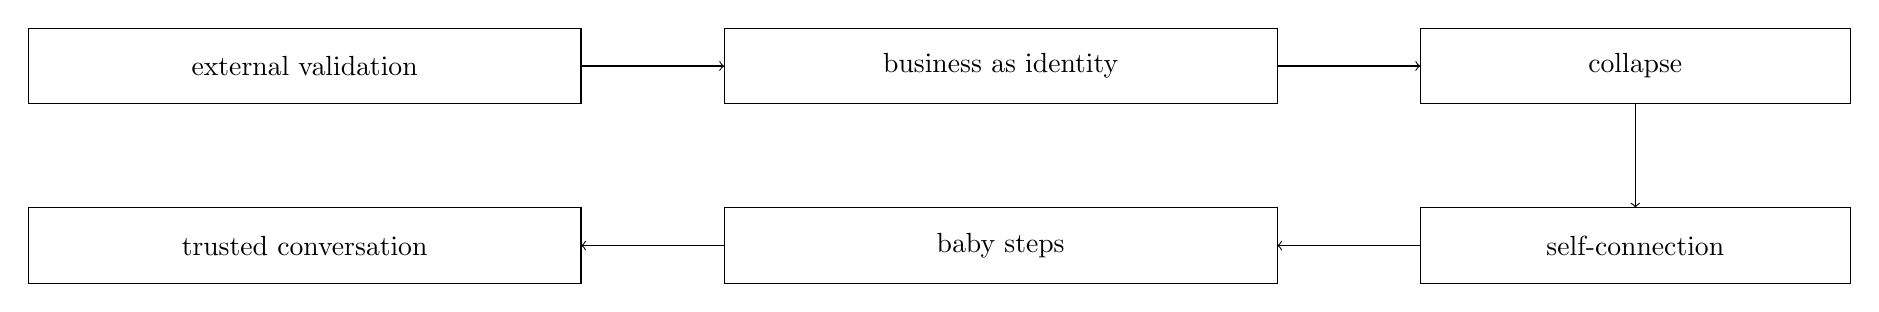
\begin{tikzpicture}[x=2.6cm,y=1.2cm]
\draw (0,0) rectangle (2.7,0.8);
\node at (1.35,0.4) {external validation};

\draw (3.4,0) rectangle (6.1,0.8);
\node at (4.75,0.4) {business as identity};

\draw (6.8,0) rectangle (8.9,0.8);
\node at (7.85,0.4) {collapse};

\draw (0,-1.9) rectangle (2.7,-1.1);
\node at (1.35,-1.5) {trusted conversation};

\draw (3.4,-1.9) rectangle (6.1,-1.1);
\node at (4.75,-1.5) {baby steps};

\draw (6.8,-1.9) rectangle (8.9,-1.1);
\node at (7.85,-1.5) {self-connection};

\draw[->] (2.7,0.4) -- (3.4,0.4);
\draw[->] (6.1,0.4) -- (6.8,0.4);
\draw[->] (7.85,0.0) -- (7.85,-1.1);
\draw[->] (6.8,-1.5) -- (6.1,-1.5);
\draw[->] (3.4,-1.5) -- (2.7,-1.5);
\end{tikzpicture}
\caption{The lecture's final inversion: outer success gives way to inner repair}
\end{figure}

\subsection{Question \& Answer}

\paragraph{Question.} What do we do when money and success stop solving the real problem?

\paragraph{Answer.} The lecture's answer is slower than its earlier business advice. We stop hiding. We talk to someone trusted. We stop mistaking sedation for healing. We accept baby steps instead of dramatic rescue. And we rebuild the self that business success had displaced. Only on that basis does the lecture allow abundance to return as something other than an anesthetic.

\section{Summary}

The lecture begins by showing us wealth at a distance and by confusing categories on purpose. It then tightens, one mechanism at a time. First access is modeled by repeated attempts. Then retail scale is modeled by margin, guarantee, simplification, and concentrated distribution. Then a tech path appears in which timing, negotiation, people, and mentors replace the retail counter as the central machine. Then entrepreneurship becomes allocation, and allocation becomes appetite for risk. Sean Mike pushes the whole lecture into its cleanest scaling logic: need-based products, delegated throughput, qualified leads, presumptive framing, and truth-telling. Finally the last interview reverses the glamour of the opening. Real estate can begin with little money; creative financing can push far beyond that; but money buys time rather than meaning, and a person who has outsourced identity to business will eventually have to rebuild from the inside outward.